
\section{Architectural design}

Many areas of our project required decisions and a rationale behind it. These decisions are sorted by area below and each decision is explained shortly. In retrospect some of these decisions were less than optimal while others turned out great and a description of how these influenced our project and what we learned will be given. The first section consists of a short overview of the system and a graphic representation. The second section talks about our database-access-layer. The third section talks about our web-framework. The fourth section is about a collection of tools for automatic code generation. The last section describes the scheduler algorithm.

\subsection{Overview}
Our system is best understood as a web-application providing the functionality to access the automatic solver and manipulate the data related to scheduling... 

\begin{figure}[H]
	\centering
		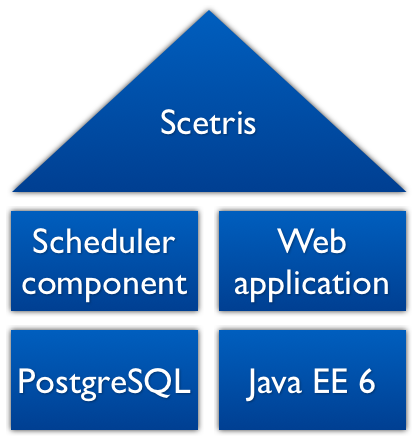
\includegraphics[width=0.5\textwidth]{images/scetris-house.png}
	\caption{\small An overview of the components}
	\label{fig:scetris-house}
\end{figure}

\subsection{Database access layer}

\emph{No existing solution but our own as we felt that existing solutions would take a similar amount of time to get used to and we would learn far more implementing the ORM ourselves. In regard to future work on the program, whether for maintenance or extension, it might prove beneficial to replace this solution with a more widely used tool, such as Hibernate. This would improve the process of understanding our software for people familiar with said tool. However we are satisfied with our own solution and we will stick with it, as it would be far too time-consuming to refactor this part of our project and we do not plan to work extensively with the software later on.}



\subsection{Web-framework}

\emph{Why we decided to use our own framework and how it is implemented. What the advantages are.}

We decided to implement our own web-framework as we wanted an easy integration of web-application and scheduling-algorithm. Thus a web-framework that uses the same language as our scheduling-algorithm was written to simplify the most common tasks. As well as getting a framework that fits our needs nicely, the benefit for us personally, which comes as knowledge was part of the reasoning against using an existing framework. We assume here that the knowledge of general principles is more beneficial to us than knowledge of tools.

\subsection{Tools for automatic code-generation}

\emph{Why a framework for common tasks has been created and how it affected our development process.}

As many tasks regarding the functionality of our web-interface require similar methods and should be implemented in a unified way to ease understanding, a framework for the most common tasks was written. It is called meta and is completely separated from the rest of our project, thus it can and will be used after we finished this project. So not only did it ease the development process for this project but also it will pay of even more in the long run.

\subsection{Scheduler Algorithm}
The problem of course scheduling problem is based on the Job-Shop Scheduling \cite{Ghaemi_usinga}. The course scheduling problem is NP-hard and the optimal solution can be found by us using heuristic search algorithm. As a matter of fact this works only for simple cases. Todays course scheduling at universities are faced with complex constraints and as the input and requirements become more complex another approach had to be considered. Based on some paper the genetic algorithm approach seemed to be promising and was chosen therefore.

\vskip 2ex

As we will not go into detail about how genetic algorithm work in general, this will be explain on the application of course scheduling in concrete. The basic data-structure to model the course scheduling problem is a set of rooms with each having a list of time slots. The components of the scheduler divide into the following:

\begin{description}
\item[Greedy Setup] generating initial population of possible solutions

\item[Fitness function] evaluating the constraint satisfaction by scoring it

\item[Crossover] creating a new possible solution by mixing course starting time slots of two possible solutions

\item[Mutation] changing a possible solution by moving randomly chosen courses to new time slots.
\end{description}

\vskip 2ex

Figure \ref{fig:scheduler} illustrates the components interaction. At the start of each scheduling a initial population containing $n$ possible schedule solutions is generated by \emph{Greedy Setup}. Randomly chosen courses are placed into the room which fits the course constraints, for instance number of seats, the best. In this step the time slots are chosen at the earliest possible time slot and are there distributed along all days at the week. If, however, there is a constraint for a preferred room or a preferred time slot entered by the main lecturer this spot is chosen instead directly.

\vskip 2ex

With the possible rise of finding a optimum schedule while generating the initial population each schedule is scored with the \emph{Fitness function} and selected into a group of best schedules. The \emph{Fitness function} is divided into two functions. A \emph{Hard fitness function} calculates a score of the hard constraint satisfaction, this includes especially solving the room-time constraint and all constraints configured to be high priority constraints. The remaining constraints are scored by a \emph{Soft fitness function}. When all constraints are satisfied an optimum schedule was found.

\begin{figure}[H]
	\centering
		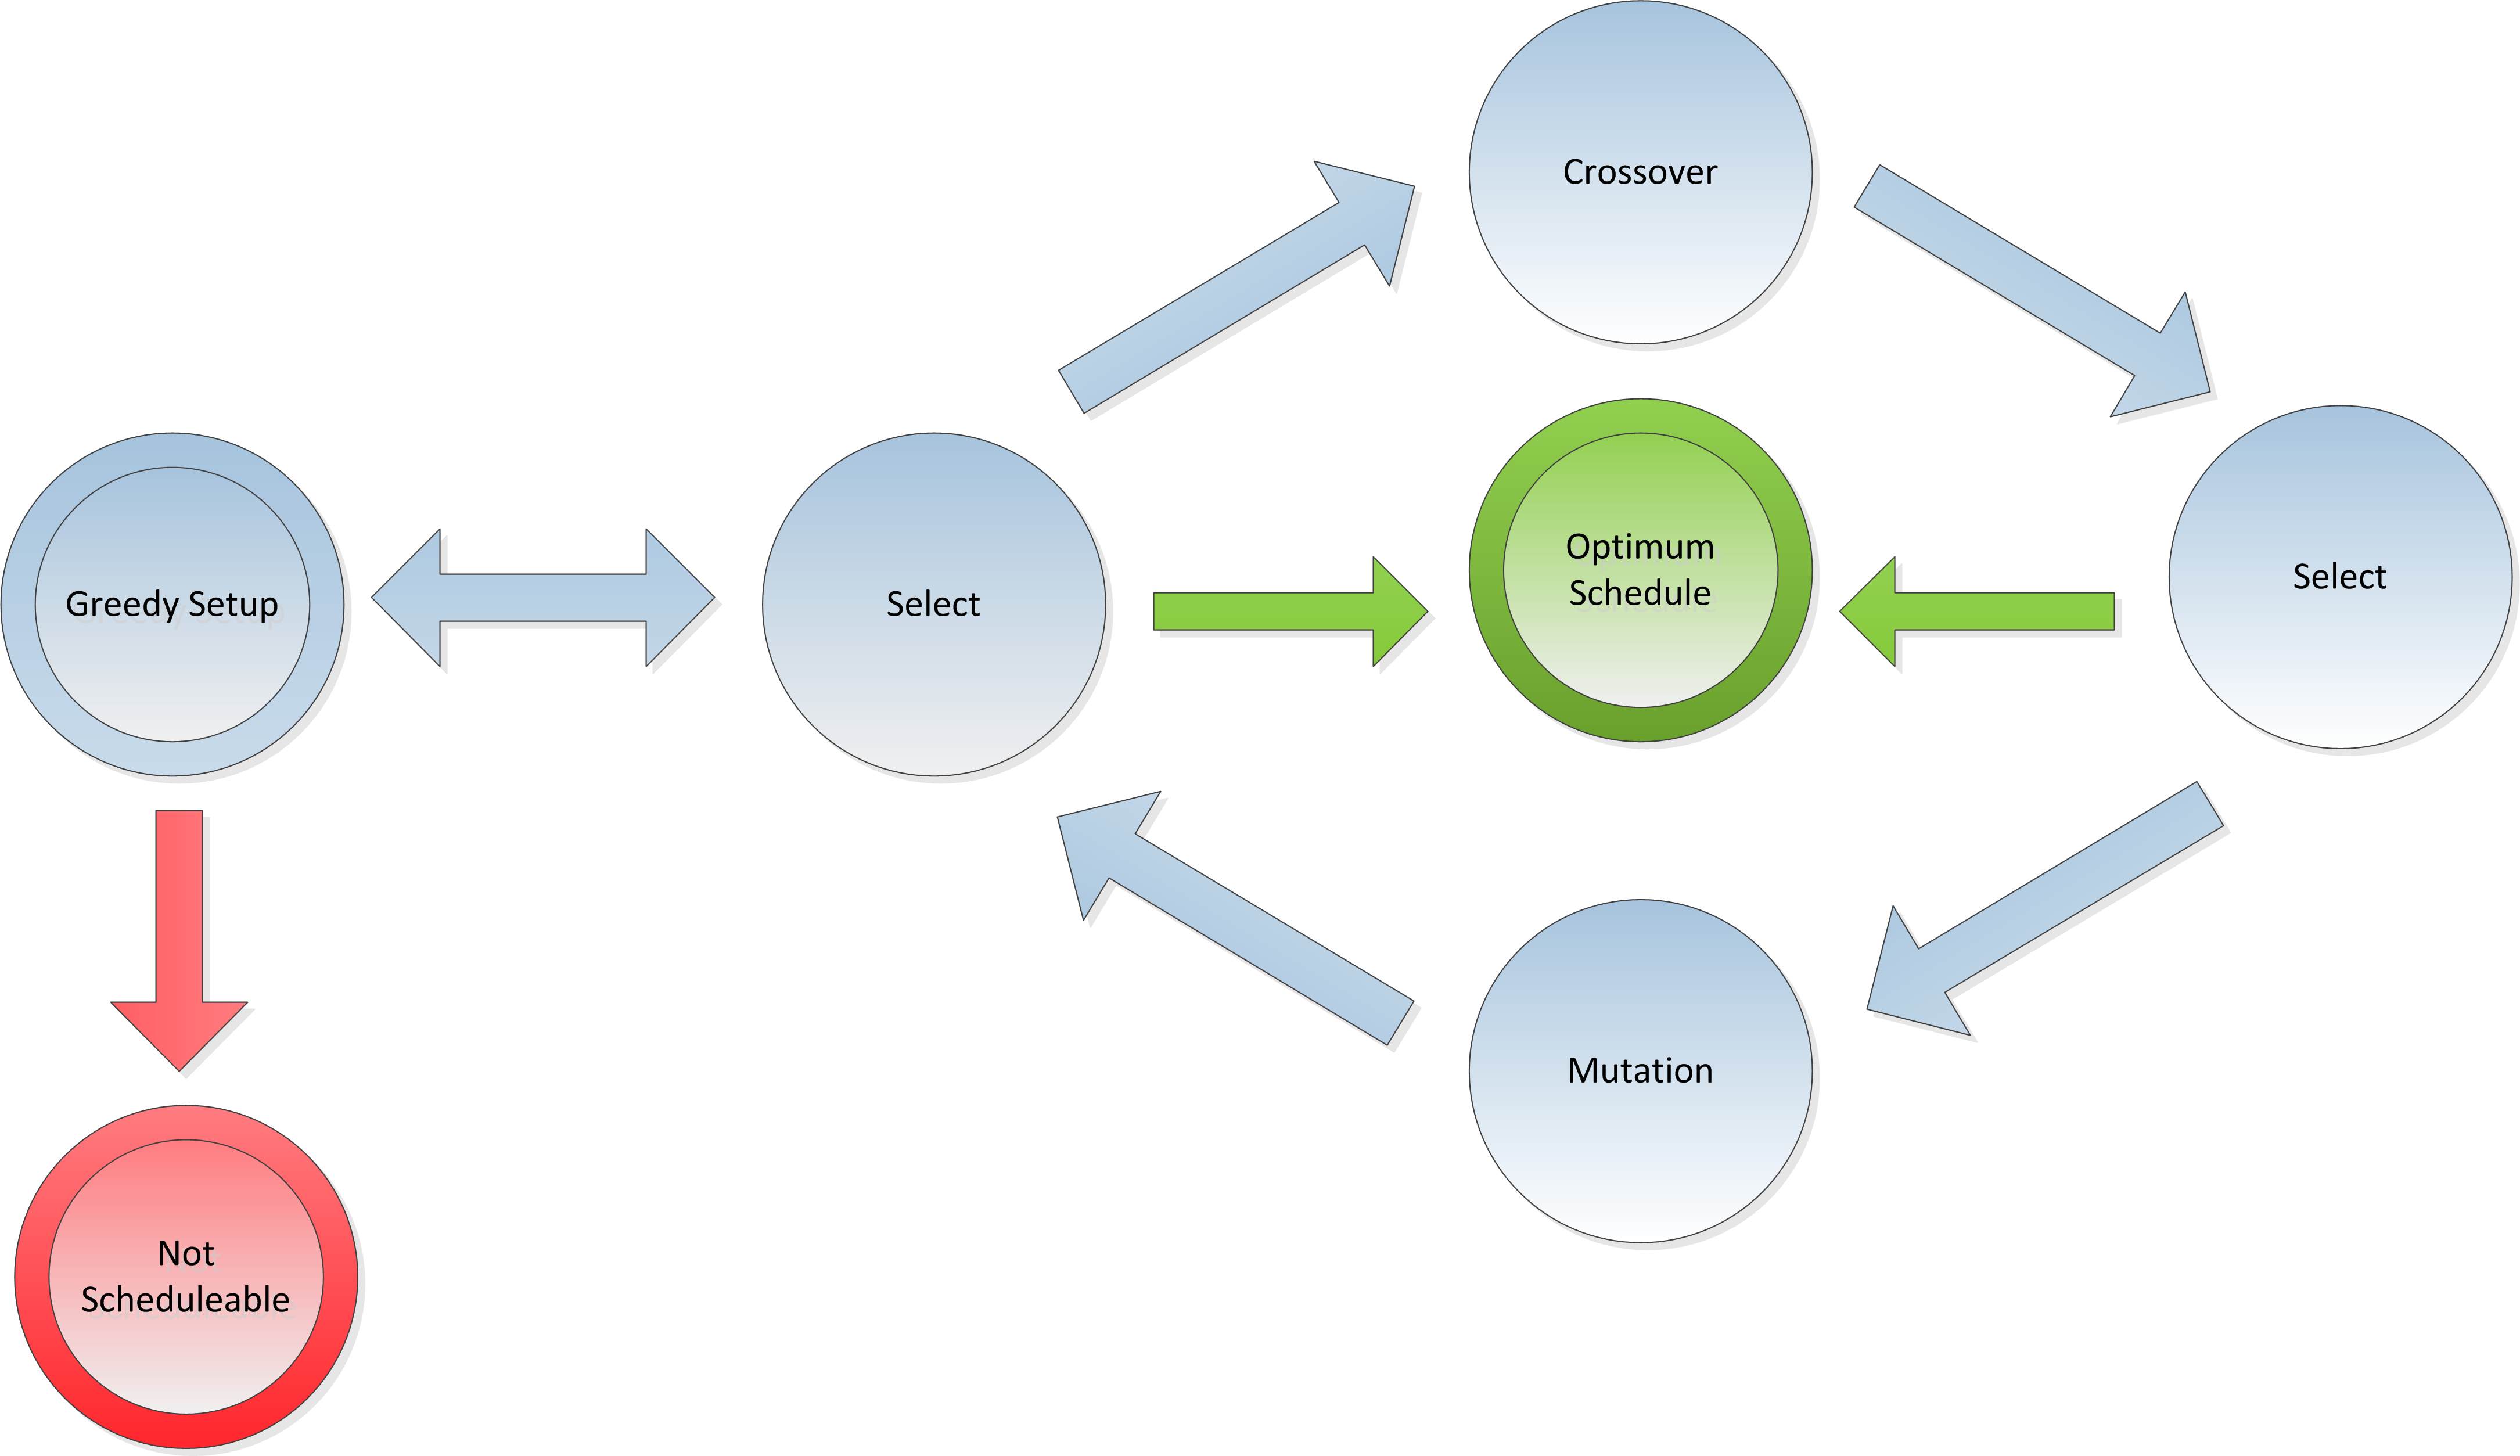
\includegraphics[width=\textwidth]{images/scheduler.png}
	\caption{Routine of the scheduler algorithm}
	\label{fig:scheduler}
\end{figure}

\vskip 2ex

Scheduling bigger input including complex constraints shows that a optimum schedule is not found in the phase of \emph{Greedy Setup}. At this point the genetic algorithm is applied. \emph{Crossover} and \emph{Mutate} is executed on the present schedules. After each operation the new schedules are evaluated by the \emph{Fitness function} until an optimum schedule was found or the scheduling is stopped by the user.
